\documentclass[border=5mm,tikz]{standalone}

\usepackage{amsmath, amssymb, amsfonts, amscd, amsthm, bigints, units}
%!TEX encoding = UTF-8 Unicode
\usepackage{tikz}
\usepackage{tikz-cd}
\usepackage{tikz3dcs-pp}
\usepackage{pgfplots}
\usepackage{xcolor, eecolors}
\usepackage{math, lrmath}

\usepackage{pgfplots}
\usepgfplotslibrary{patchplots}
\pgfplotsset{compat=1.15}

\usetikzlibrary{calc, intersections}

\usetikzlibrary{decorations.pathmorphing,calc,shapes,positioning,fit,arrows,fadings,decorations.pathreplacing,decorations.pathmorphing,intersections,patterns, trees}
\usetikzlibrary{decorations.markings}

\usepackage{marvosym}

%%%%%%%%My Tikz definitions%%%%%%%%%%%%%%%%%
\tikzset{->-/.style={decoration={
  markings,
  mark=at position #1 with {\arrow{latex}}},postaction={decorate}}}
  %
\tikzset{
    %Define standard arrow tip
    >=stealth',
    %Define style for boxes
    punkt/.style={
           rectangle,
           rounded corners,
           draw=black, very thick,
           text width=7.5em,
           minimum height=2em,
           text centered},
    % Define arrow style
    pil/.style={
           ->,
           thick,
           shorten <=2pt,
           shorten >=2pt,}
}
%%%
%%3d drawings %%%
\newcommand\pgfmathsinandcos[3]{%
  \pgfmathsetmacro#1{sin(#3)}%
  \pgfmathsetmacro#2{cos(#3)}%
}
\newcommand\LongitudePlane[3][current plane]{%
  \pgfmathsinandcos\sinEl\cosEl{#2} % elevation
  \pgfmathsinandcos\sint\cost{#3} % azimuth
  \tikzset{#1/.style={cm={\cost,\sint*\sinEl,0,\cosEl,(0,0)}}}
}
\newcommand\LatitudePlane[3][current plane]{%
  \pgfmathsinandcos\sinEl\cosEl{#2} % elevation
  \pgfmathsinandcos\sint\cost{#3} % latitude
  \pgfmathsetmacro\yshift{\cosEl*\sint}
  \tikzset{#1/.style={cm={\cost,0,0,\cost*\sinEl,(0,\yshift)}}} %
}
\newcommand\DrawLongitudeCircle[2][1]{
  \LongitudePlane{\angEl}{#2}
  \tikzset{current plane/.prefix style={scale=#1}}
   % angle of "visibility"
  \pgfmathsetmacro\angVis{atan(sin(#2)*cos(\angEl)/sin(\angEl))} %
  \draw[current plane] (\angVis:1) arc (\angVis:\angVis+180:1);
  \draw[current plane,dashed] (\angVis-180:1) arc (\angVis-180:\angVis:1);
}
\newcommand\DrawLatitudeCircle[2][1]{
  \LatitudePlane{\angEl}{#2}
  \tikzset{current plane/.prefix style={scale=#1}}
  \pgfmathsetmacro\sinVis{sin(#2)/cos(#2)*sin(\angEl)/cos(\angEl)}
  % angle of "visibility"
  \pgfmathsetmacro\angVis{asin(min(1,max(\sinVis,-1)))}
  \draw[current plane] (\angVis:1) arc (\angVis:-\angVis-180:1);
  \draw[current plane,dashed] (180-\angVis:1) arc (180-\angVis:\angVis:1);
}
%%%%


\begin{document}
				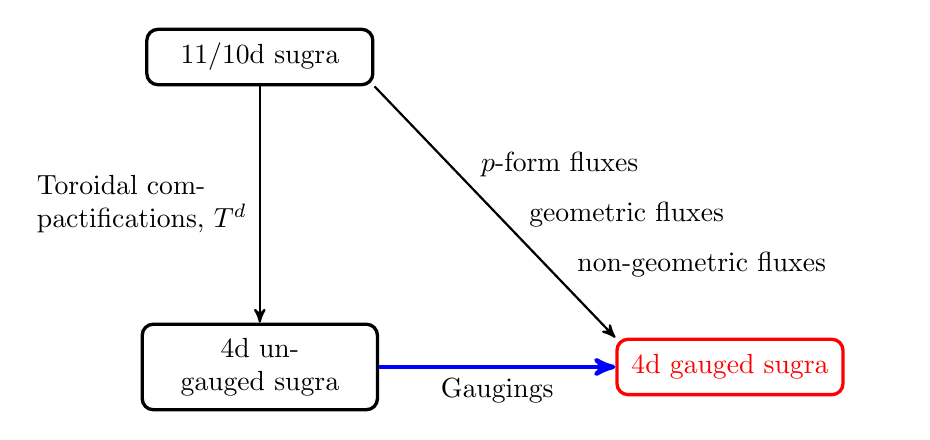
\begin{tikzpicture}
				%
					%nodes
					\node[punkt] (Msugra) {$11$/$10$d sugra};
					\node[punkt, inner sep=5pt,below=3cm of Msugra] (4sugra) {$4$d ungauged sugra};
					\node[punkt, below=3cm of Msugra, right=3cm of 4sugra, color=red] (gaugedsugra) {$4$d gauged sugra};
					%drawings
					\draw[->, thick] (Msugra.south) -- (4sugra.north)
						node[pos=0.5, left, text width = 2.7cm] {Toroidal compactifications, $T^d$};
					%
					\draw[->, color=blue, ultra thick] (4sugra.east) -- (gaugedsugra.west)
						node[pos=0.5, below, color = black] {Gaugings};
					%
					\draw[->, thick] (Msugra.south east) -- (gaugedsugra.north west)
						node[pos=0.4, above right, text width = 2.5cm] {$p$-form fluxes}
						node[pos=0.6, above right, text width = 3cm] {geometric fluxes}
						node[pos=0.8, above right, text width = 4cm] {non-geometric fluxes};
				%
				\end{tikzpicture}
\end{document}